\documentclass[aspectratio=169,11pt]{beamer}

\usetheme{Madrid}
\usecolortheme{default}

% ── Packages ──────────────────────────────────────────────────────
\usepackage[utf8]{inputenc}
\usepackage[T1]{fontenc}
\usepackage{amsmath,amssymb}
\usepackage{booktabs}
\usepackage{graphicx}
\usepackage{listings}
\usepackage{xcolor}
\usepackage{tikz}
\usetikzlibrary{arrows.meta, positioning, shapes.geometric, calc}
\usepackage{hyperref}

% ── Code listing style ───────────────────────────────────────────
\definecolor{codebg}{HTML}{F5F5F0}
\definecolor{codegreen}{HTML}{2E7D32}
\definecolor{codegray}{HTML}{808080}
\definecolor{codepurple}{HTML}{7B1FA2}
\definecolor{codeblue}{HTML}{1565C0}

\lstdefinestyle{py}{
  language=Python,
  backgroundcolor=\color{codebg},
  basicstyle=\ttfamily\scriptsize,
  keywordstyle=\color{codeblue}\bfseries,
  commentstyle=\color{codegray}\itshape,
  stringstyle=\color{codegreen},
  emphstyle=\color{codepurple},
  showstringspaces=false,
  breaklines=true,
  frame=single,
  rulecolor=\color{gray!40},
  xleftmargin=4pt,
  xrightmargin=4pt,
  aboveskip=6pt,
  belowskip=4pt,
  columns=flexible,
  morekeywords={self,True,False,None,as,with,yield,lambda},
}
\lstset{style=py}

% ── Metadata ─────────────────────────────────────────────────────
\title[Chapter 1 -- Lab Session]{%
  Chapter 1 Lab -- Text as Data:\\
  TF-IDF and Document Similarity on SEC Filings}
\subtitle{Advanced Machine Learning for Finance}
\author{Giovanni Della Lunga}
\institute{University of Bologna}
\date{April--May 2026}

% ══════════════════════════════════════════════════════════════════
\begin{document}

% ── Title ─────────────────────────────────────────────────────────
\begin{frame}
\titlepage
\end{frame}

% ── Objectives ────────────────────────────────────────────────────
\begin{frame}{Lab Objectives}

This notebook applies the concepts from Lesson~1 to
\textbf{real financial text} drawn from the SEC EDGAR database:

\begin{enumerate}
  \item \textbf{Corpus construction} -- fetch 10-K annual filings
        from EDGAR for companies across different sectors.
  \item \textbf{Preprocessing} -- compare classical tokenization with
        subword (BPE) tokenization; examine the effect of stop-word
        removal, stemming, and lemmatization.
  \item \textbf{TF-IDF representation} -- build sparse vectors
        using scikit-learn and inspect distinctive terms.
  \item \textbf{Document similarity} -- compute and visualize cosine
        similarity; compare it with Euclidean distance.
  \item \textbf{Critical analysis} -- identify where TF-IDF succeeds
        and where it fails.
\end{enumerate}

\end{frame}

% ── Roadmap ───────────────────────────────────────────────────────
\begin{frame}{Roadmap}
\tableofcontents
\end{frame}

% ══════════════════════════════════════════════════════════════════
\section{Building a Corpus from SEC EDGAR}
% ══════════════════════════════════════════════════════════════════

\begin{frame}{SEC EDGAR: The Data Source}

\begin{itemize}
  \item The U.S.\ Securities and Exchange Commission maintains
        \textbf{EDGAR} (Electronic Data Gathering, Analysis,
        and Retrieval).
  \item EDGAR is the main public repository for corporate
        regulatory filings in the United States.
  \item Researchers can access annual reports (Form~10-K),
        quarterly reports (Form~10-Q), and many other disclosures.
  \item In this lab we use the Python library \texttt{EdgarTools}
        to interact with EDGAR programmatically.
\end{itemize}

\vspace{6pt}
\begin{block}{Focus section}
We extract the \textbf{Risk Factors} section (Item~1A) from
each 10-K filing --- a narrative section rich in domain-specific
language.
\end{block}

\end{frame}

% ──────────────────────────────────────────────────────────────────
\begin{frame}{Company Selection}

\small
\begin{table}
\centering
\begin{tabular}{llll}
\toprule
\textbf{Ticker} & \textbf{Company} & \textbf{Sector} \\
\midrule
JPM   & JPMorgan Chase      & Banking           \\
GS    & Goldman Sachs        & Banking           \\
BAC   & Bank of America      & Banking           \\
AAPL  & Apple                & Technology        \\
MSFT  & Microsoft            & Technology        \\
GOOGL & Alphabet             & Technology        \\
XOM   & ExxonMobil           & Energy            \\
CVX   & Chevron              & Energy            \\
PFE   & Pfizer               & Healthcare        \\
JNJ   & Johnson \& Johnson   & Healthcare        \\
KO    & Coca-Cola            & Consumer Staples  \\
PG    & Procter \& Gamble    & Consumer Staples  \\
\bottomrule
\end{tabular}
\end{table}

\vspace{4pt}
\textbf{Design:} 12 companies $\times$ 5 sectors. Same-sector
companies should cluster together under TF-IDF similarity;
cross-sector pairs should not.

\end{frame}

% ──────────────────────────────────────────────────────────────────
\begin{frame}[fragile]{Fetching Filing Metadata from EDGAR}

\begin{lstlisting}
def get_latest_10k_url(cik):
    """Fetch the URL of the most recent 10-K
       filing for a given company CIK."""
    url = f"https://data.sec.gov/submissions/CIK{cik:010d}.json"
    resp = requests.get(url, headers=HEADERS)
    resp.raise_for_status()
    data = resp.json()
    recent = data['filings']['recent']
    for i, form in enumerate(recent['form']):
        if form == '10-K':
            acc = recent['accessionNumber'][i].replace('-', '')
            doc = recent['primaryDocument'][i]
            return (f"https://www.sec.gov/Archives/edgar/"
                    f"data/{cik}/{acc}/{doc}",
                    recent['accessionNumber'][i])
    return None, None
\end{lstlisting}

\begin{block}{Key point}
The SEC API requires a valid \texttt{User-Agent} header and
rate-limiting (max 10~requests/second).
\end{block}

\end{frame}

% ──────────────────────────────────────────────────────────────────
\begin{frame}[fragile]{Extracting Risk Factors Text}

\begin{lstlisting}
from edgar import Company

def extract_text_from_filing(cik, max_chars=None):
    """Extract Risk Factors (Item 1A) from the latest 10-K."""
    company = Company(str(cik))
    filing = company.get_filings(form="10-K").latest()
    tenk = filing.obj()
    text = getattr(tenk, "risk_factors", None)
    if not text:
        text = tenk["Item 1A"]  # fallback
    text = re.sub(r"\s+", " ", str(text)).strip()
    return text[:max_chars] if max_chars else text
\end{lstlisting}

\vspace{6pt}
\small
\begin{block}{Corpus statistics}
12 documents, ranging from $\sim$34\,000 chars (CVX)
to $\sim$142\,000 chars (GS).
Approximate token counts: 5\,000--21\,000 tokens per document.
\end{block}

\end{frame}

% ══════════════════════════════════════════════════════════════════
\section{Preprocessing}
% ══════════════════════════════════════════════════════════════════

\begin{frame}{Classical vs.\ BPE Tokenization}

\begin{columns}[T]
\begin{column}{0.48\textwidth}
\textbf{Classical tokenization}\\[4pt]
Split on whitespace and punctuation; lowercase.
\vspace{4pt}

\small
\texttt{jpmorganchase, must, periodically, submit, a, detailed,
resolution, plan, to, the, federal, reserve, \ldots}

\vspace{6pt}
$\rightarrow$ 39 tokens
\end{column}
\begin{column}{0.48\textwidth}
\textbf{BPE tokenization (GPT-4)}\\[4pt]
Subword segmentation using byte-pair encoding.
\vspace{4pt}

\small
\texttt{J, PM, organ, Ch, ase, \ must, \ periodically, \ submit,
\ a, \ detailed, \ resolution, \ plan, \ldots}

\vspace{6pt}
$\rightarrow$ 44 tokens
\end{column}
\end{columns}

\vspace{8pt}
\begin{alertblock}{Observation}
BPE splits financial terms into semantically
meaningless fragments: \texttt{FDIC}~$\to$~\texttt{FD|IC},
\texttt{EBITDA}~$\to$~\texttt{EB|IT|DA}.
This is one reason why LLMs struggle with arithmetic and
precise entity matching.
\end{alertblock}

\end{frame}

% ──────────────────────────────────────────────────────────────────
\begin{frame}[fragile]{The Preprocessing Pipeline}

\begin{lstlisting}
stemmer    = PorterStemmer()
lemmatizer = WordNetLemmatizer()
stop_words = set(stopwords.words('english'))

def preprocess(text, remove_stops=False,
               do_stem=False, do_lemma=False):
    tokens = word_tokenize(text.lower())
    tokens = [t for t in tokens if t.isalpha() and len(t) > 2]
    if remove_stops:
        tokens = [t for t in tokens if t not in stop_words]
    if do_stem:
        tokens = [stemmer.stem(t) for t in tokens]
    elif do_lemma:
        tokens = [lemmatizer.lemmatize(t) for t in tokens]
    return ' '.join(tokens)
\end{lstlisting}

\vspace{4pt}
We build \textbf{four} versions of the corpus:
\texttt{raw}, \texttt{no\_stopwords}, \texttt{stemmed},
\texttt{lemmatized}.

\end{frame}

% ──────────────────────────────────────────────────────────────────
\begin{frame}{The Effect of Preprocessing Choices}

\begin{table}
\centering
\begin{tabular}{lrr}
\toprule
\textbf{Version} & \textbf{Vocab size} & \textbf{Avg tokens/doc} \\
\midrule
raw            & 5{,}462 & 8{,}893 \\
no\_stopwords  & 5{,}377 & 6{,}560 \\
stemmed        & 3{,}059 & 6{,}560 \\
lemmatized     & 4{,}615 & 6{,}560 \\
\bottomrule
\end{tabular}
\end{table}

\vspace{6pt}
\begin{itemize}
  \item Each preprocessing step \textbf{reduces} the vocabulary size
        --- this is a form of information compression.
  \item Stemming is the most aggressive single step.
  \item The question is always: \textbf{does the removed information
        matter for the task?}
\end{itemize}

\begin{exampleblock}{Task dependence}
For document-level similarity, removing stop words typically helps.
For sentiment analysis, removing ``not'' can invert the meaning
of a sentence.
\end{exampleblock}

\end{frame}

% ══════════════════════════════════════════════════════════════════
\section{TF-IDF Representation}
% ══════════════════════════════════════════════════════════════════

\begin{frame}[fragile]{Building the TF-IDF Matrix}

We use the \textbf{lemmatized, stop-word-free} version of the
corpus --- the version that best balances vocabulary reduction
with semantic preservation.

\begin{lstlisting}
tfidf = TfidfVectorizer(
    max_features = 5000,   # keep top 5000 terms
    min_df       = 2,      # term must appear in >= 2 docs
    max_df       = 0.95,   # ignore terms in > 95% of docs
    sublinear_tf = False,  # raw TF, to match lecture
    norm         = 'l2',   # L2 normalization (standard)
)
tfidf_matrix = tfidf.fit_transform(docs_for_tfidf)
\end{lstlisting}

\vspace{6pt}
\begin{block}{Result}
TF-IDF matrix shape: $12 \times 2{,}584$.
Density: $\sim$39.5\,\% --- approximately 60\,\% of entries
are zero. This is a \textbf{sparse representation}.
\end{block}

\end{frame}

% ──────────────────────────────────────────────────────────────────
\begin{frame}[fragile]{Most Distinctive Terms per Company}

\begin{lstlisting}
def top_tfidf_terms(matrix, feature_names, doc_index, n=10):
    row = matrix[doc_index].toarray().flatten()
    top_idx = row.argsort()[::-1][:n]
    return [(feature_names[i], round(row[i], 3))
            for i in top_idx]
\end{lstlisting}

\vspace{6pt}
For each document we extract the terms with the highest
TF-IDF weight --- terms that are \textbf{frequent in that
document} but \textbf{rare across the corpus}.

\vspace{6pt}
\begin{block}{The IDF mechanism at work}
Terms like \emph{revenue} or \emph{operating} are common
across all 10-K filings $\Rightarrow$ low IDF weight.
Terms like \emph{drilling} or \emph{pharmaceutical} are
sector-specific $\Rightarrow$ high IDF weight
$\Rightarrow$ high TF-IDF score.
\end{block}

\end{frame}

% ──────────────────────────────────────────────────────────────────
\begin{frame}{Interpreting the Top Terms}

\begin{columns}[T]
\begin{column}{0.48\textwidth}
\textbf{Expected patterns:}
\begin{itemize}
  \item \textbf{Banking} companies share terms
        such as \emph{loan}, \emph{deposit},
        \emph{credit}, \emph{interest}.
  \item \textbf{Technology} companies share
        terms such as \emph{cloud}, \emph{user},
        \emph{advertising}.
  \item \textbf{Energy} companies share terms
        such as \emph{oil}, \emph{drilling},
        \emph{exploration}.
\end{itemize}
\end{column}
\begin{column}{0.48\textwidth}
\textbf{What to watch for:}
\begin{itemize}
  \item Cross-sector overlap: terms like
        \emph{regulatory} or \emph{compliance}
        may appear across sectors.
  \item Company-specific terms: \emph{iPhone}
        for AAPL, \emph{Azure} for MSFT.
  \item The IDF component suppresses terms
        that are too ubiquitous.
\end{itemize}
\end{column}
\end{columns}

\vspace{8pt}
\begin{block}{Key idea}
TF-IDF automatically surfaces \textbf{discriminative}
vocabulary --- precisely the terms that distinguish one
document from another.
\end{block}

\end{frame}

% ══════════════════════════════════════════════════════════════════
\section{Document Similarity}
% ══════════════════════════════════════════════════════════════════

\begin{frame}[fragile]{Cosine Similarity Matrix}

\begin{lstlisting}
cos_sim = cosine_similarity(tfidf_matrix)
cos_df  = pd.DataFrame(cos_sim, index=tickers, columns=tickers)
\end{lstlisting}

\vspace{6pt}
The result is a $12 \times 12$ matrix where entry $(i,j)$
records the cosine similarity between the TF-IDF vectors
of companies $i$ and $j$.

\vspace{6pt}
\begin{itemize}
  \item Diagonal entries $= 1$ (each document is identical
        to itself).
  \item Off-diagonal entries $\in [0,1]$ (all TF-IDF weights
        are non-negative).
  \item We visualize this as a \textbf{heatmap} with
        color-coded sector labels.
\end{itemize}

\end{frame}

% ──────────────────────────────────────────────────────────────────
\begin{frame}{Heatmap Visualization}

\begin{center}
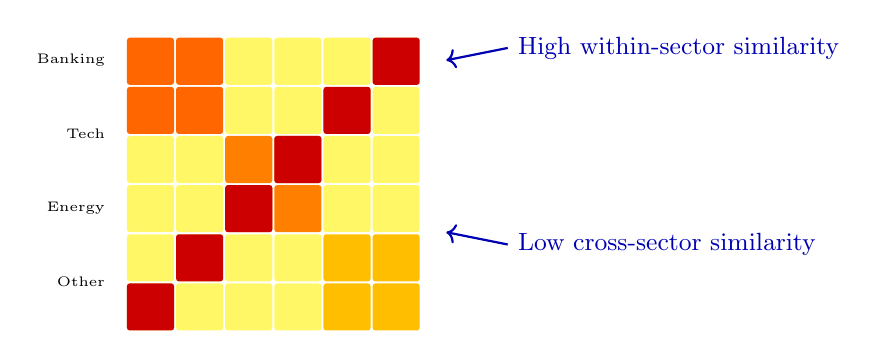
\begin{tikzpicture}[scale=0.52, every node/.style={font=\tiny}]
% Draw a schematic 6x6 heatmap representing sector blocks
\def\cellsize{1.2}

% Sector labels
\node[rotate=0, anchor=east] at (-0.3, 5*\cellsize+0.6) {Banking};
\node[rotate=0, anchor=east] at (-0.3, 3.5*\cellsize+0.6) {Tech};
\node[rotate=0, anchor=east] at (-0.3, 2*\cellsize+0.6) {Energy};
\node[rotate=0, anchor=east] at (-0.3, 0.5*\cellsize+0.6) {Other};

% High-sim blocks (within sector) - darker
\foreach \r in {4,5} {
  \foreach \c in {0,1} {
    \fill[red!60!yellow, rounded corners=1pt]
      (\c*\cellsize, \r*\cellsize)
      rectangle +(\cellsize-0.05, \cellsize-0.05);
  }
}

\foreach \r in {2,3} {
  \foreach \c in {2,3} {
    \fill[red!50!yellow, rounded corners=1pt]
      (\c*\cellsize, \r*\cellsize)
      rectangle +(\cellsize-0.05, \cellsize-0.05);
  }
}

% Low-sim blocks (across sector) - lighter
\foreach \r in {4,5} {
  \foreach \c in {2,3,4,5} {
    \fill[yellow!60!white, rounded corners=1pt]
      (\c*\cellsize, \r*\cellsize)
      rectangle +(\cellsize-0.05, \cellsize-0.05);
  }
}
\foreach \r in {2,3} {
  \foreach \c in {0,1,4,5} {
    \fill[yellow!60!white, rounded corners=1pt]
      (\c*\cellsize, \r*\cellsize)
      rectangle +(\cellsize-0.05, \cellsize-0.05);
  }
}

\foreach \r in {0,1} {
  \foreach \c in {4,5} {
    \fill[orange!50!yellow, rounded corners=1pt]
      (\c*\cellsize, \r*\cellsize)
      rectangle +(\cellsize-0.05, \cellsize-0.05);
  }
}
\foreach \r in {0,1} {
  \foreach \c in {0,1,2,3} {
    \fill[yellow!60!white, rounded corners=1pt]
      (\c*\cellsize, \r*\cellsize)
      rectangle +(\cellsize-0.05, \cellsize-0.05);
  }
}

% Diagonal
\foreach \i in {0,...,5} {
  \fill[red!80!black, rounded corners=1pt]
    (\i*\cellsize, \i*\cellsize)
    rectangle +(\cellsize-0.05, \cellsize-0.05);
}

% Annotations
\draw[<-, thick, blue!70!black]
  (7.8, 5.5*\cellsize) -- ++(1.5, 0.3)
  node[right, font=\small] {High within-sector similarity};
\draw[<-, thick, blue!70!black]
  (7.8, 2*\cellsize) -- ++(1.5, -0.3)
  node[right, font=\small] {Low cross-sector similarity};

\end{tikzpicture}
\end{center}

\vspace{4pt}
\begin{block}{Expected pattern}
Within-sector blocks show \textbf{higher} cosine similarity
than cross-sector blocks, confirming that companies in the same
industry share domain-specific vocabulary in their Risk Factors.
\end{block}

\end{frame}

% ──────────────────────────────────────────────────────────────────
\begin{frame}[fragile]{Do Companies Cluster by Sector?}

\begin{lstlisting}
within_sector = []
across_sector = []
for i in range(len(tickers)):
    for j in range(i+1, len(tickers)):
        sim = cos_sim[i, j]
        if COMPANIES[tickers[i]]['sector'] == \
           COMPANIES[tickers[j]]['sector']:
            within_sector.append(sim)
        else:
            across_sector.append(sim)
\end{lstlisting}

\vspace{6pt}
\begin{columns}[c]
\begin{column}{0.45\textwidth}
\centering
\textbf{Within sector}\\[4pt]
Higher average cosine\\
($n = 11$ pairs)
\end{column}
\begin{column}{0.1\textwidth}
\centering
\Large $\gg$
\end{column}
\begin{column}{0.45\textwidth}
\centering
\textbf{Across sectors}\\[4pt]
Lower average cosine\\
($n = 55$ pairs)
\end{column}
\end{columns}

\vspace{6pt}
\begin{block}{Conclusion}
TF-IDF similarity correctly separates same-sector from
cross-sector document pairs in this corpus.
\end{block}

\end{frame}

% ──────────────────────────────────────────────────────────────────
\begin{frame}{Euclidean Distance vs.\ Cosine Similarity}

Recall from the lecture that Euclidean distance conflates
\textbf{what} a document is about (direction) with
\textbf{how long} it is (magnitude).

\vspace{8pt}
\begin{columns}[T]
\begin{column}{0.48\textwidth}
\textbf{Cosine similarity}
\begin{itemize}
  \item Compares directions only.
  \item Within-sector pairs score high.
  \item Length-invariant.
\end{itemize}
\end{column}
\begin{column}{0.48\textwidth}
\textbf{Euclidean distance}
\begin{itemize}
  \item Mixes direction and magnitude.
  \item A short and a long document on the
        same topic may appear distant.
  \item Sector structure is blurred.
\end{itemize}
\end{column}
\end{columns}

\vspace{8pt}
\begin{alertblock}{Empirical verification}
When we compute both metrics on the same TF-IDF matrix, the
sector clustering visible under cosine similarity becomes
less clear under Euclidean distance ---
confirming the theoretical argument from the lecture.
\end{alertblock}

\end{frame}

% ──────────────────────────────────────────────────────────────────
\begin{frame}{Visualizing the Document Space}

\begin{columns}[T]
\begin{column}{0.55\textwidth}

We reduce the TF-IDF vectors to 2~dimensions using
\textbf{Truncated SVD} (related to PCA for sparse matrices).

\vspace{6pt}
\begin{itemize}
  \item Each dot is a company.
  \item Colors indicate sectors.
  \item Companies in the same sector cluster together.
\end{itemize}

\vspace{6pt}
\begin{block}{What SVD captures}
The first two components span the directions of
maximum variance in the TF-IDF space. Sector
separation along these axes confirms that the
vocabulary structure encodes industry identity.
\end{block}

\end{column}
\begin{column}{0.42\textwidth}

\centering
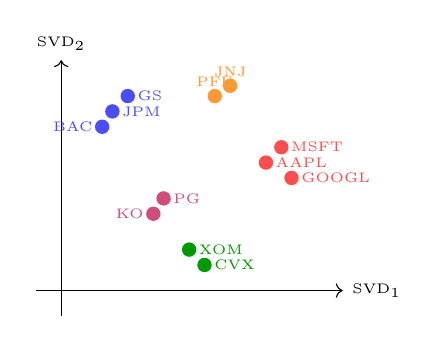
\begin{tikzpicture}[scale=0.65]
  \draw[->] (-0.5,0) -- (5.5,0) node[right] {\tiny SVD$_1$};
  \draw[->] (0,-0.5) -- (0,4.5) node[above] {\tiny SVD$_2$};

  % Banking cluster
  \fill[blue!70] (1.0,3.5) circle (4pt) node[right,font=\tiny]{JPM};
  \fill[blue!70] (1.3,3.8) circle (4pt) node[right,font=\tiny]{GS};
  \fill[blue!70] (0.8,3.2) circle (4pt) node[left,font=\tiny]{BAC};

  % Tech cluster
  \fill[red!70] (4.0,2.5) circle (4pt) node[right,font=\tiny]{AAPL};
  \fill[red!70] (4.3,2.8) circle (4pt) node[right,font=\tiny]{MSFT};
  \fill[red!70] (4.5,2.2) circle (4pt) node[right,font=\tiny]{GOOGL};

  % Energy cluster
  \fill[green!60!black] (2.5,0.8) circle (4pt) node[right,font=\tiny]{XOM};
  \fill[green!60!black] (2.8,0.5) circle (4pt) node[right,font=\tiny]{CVX};

  % Healthcare
  \fill[orange!80] (3.0,3.8) circle (4pt) node[above,font=\tiny]{PFE};
  \fill[orange!80] (3.3,4.0) circle (4pt) node[above,font=\tiny]{JNJ};

  % Consumer
  \fill[purple!70] (1.8,1.5) circle (4pt) node[left,font=\tiny]{KO};
  \fill[purple!70] (2.0,1.8) circle (4pt) node[right,font=\tiny]{PG};
\end{tikzpicture}

\vspace{2pt}
{\tiny Schematic illustration of the SVD projection}

\end{column}
\end{columns}

\end{frame}

% ══════════════════════════════════════════════════════════════════
\section{Critical Analysis}
% ══════════════════════════════════════════════════════════════════

\begin{frame}{Where TF-IDF Succeeds}

\begin{itemize}
  \item \textbf{Same-sector clustering}: companies in the same
        industry share domain-specific vocabulary
        (\emph{loan}, \emph{deposit} for banks;
         \emph{cloud}, \emph{user} for tech firms).
  \item \textbf{Discriminative terms}: TF-IDF automatically
        surfaces the vocabulary that distinguishes each
        company or sector from the rest of the corpus.
  \item \textbf{Interpretability}: every dimension of the
        TF-IDF vector corresponds to a known word, making
        it easy to explain why two documents are similar.
\end{itemize}

\vspace{6pt}
\begin{block}{Practical relevance}
TF-IDF remains a strong baseline for document retrieval,
topic analysis, and exploratory text mining on financial
corpora.
\end{block}

\end{frame}

% ──────────────────────────────────────────────────────────────────
\begin{frame}{Where TF-IDF Fails}

TF-IDF similarity requires \textbf{lexical overlap}: two
documents can only be similar if they share the same words.

\vspace{6pt}
\begin{alertblock}{The semantic gap}
\small
\begin{tabular}{ll}
Sentence A: & \emph{The company implemented a cost reduction program.}\\
Sentence B: & \emph{The firm executed an expense cutting initiative.}\\
\end{tabular}

\vspace{4pt}
A human reader sees these as nearly identical in meaning.
After stop-word removal, their TF-IDF vectors share
\textbf{zero terms} $\Rightarrow$ cosine similarity
$= 0$.
\end{alertblock}

\vspace{6pt}
Systematic blind spots include:

\begin{itemize}
  \item \textbf{Synonymy}: ``cost reduction'' vs.\ ``expense cutting.''
  \item \textbf{Paraphrase}: same idea, entirely different wording.
  \item \textbf{Cross-domain similarity}: two sectors facing
        structurally similar risks described with different vocabulary.
\end{itemize}

\end{frame}

% ──────────────────────────────────────────────────────────────────
\begin{frame}[fragile]{Demonstrating the Semantic Gap}

\begin{lstlisting}
pair_a = "The company implemented a cost reduction program"
pair_b = "The firm executed an expense cutting initiative"

v_a = tfidf.transform([preprocess(pair_a,
          remove_stops=True, do_lemma=True)])
v_b = tfidf.transform([preprocess(pair_b,
          remove_stops=True, do_lemma=True)])

sim = cosine_similarity(v_a, v_b)[0, 0]

print(f"Cosine similarity (TF-IDF): {sim:.3f}")
# Output: 0.000
\end{lstlisting}

\vspace{6pt}
\begin{block}{The fundamental limitation}
TF-IDF captures \textbf{lexical co-occurrence}, not
\textbf{semantic meaning}. This is the core limitation
that motivates the transition to \textbf{dense
representations} (embeddings).
\end{block}

\end{frame}

% ──────────────────────────────────────────────────────────────────
\begin{frame}[fragile]{Explaining Similarity: Shared Terms}

\begin{lstlisting}
def explain_similarity(t1, t2, matrix, feature_names,
                       tickers, top_n=10):
    v1 = matrix[tickers.index(t1)].toarray().flatten()
    v2 = matrix[tickers.index(t2)].toarray().flatten()
    contrib = v1 * v2  # element-wise (dot-product terms)
    top_idx = contrib.argsort()[::-1][:top_n]
    for idx in top_idx:
        if contrib[idx] > 0:
            print(f"  {feature_names[idx]:<20s}  "
                  f"product = {contrib[idx]:.4f}")
\end{lstlisting}

\vspace{6pt}
\begin{itemize}
  \item High-similarity pairs share \textbf{content terms}:
        banking pairs share \emph{loan}, \emph{credit},
        \emph{deposit}.
  \item Low-similarity pairs share only \textbf{generic terms}:
        \emph{risk}, \emph{business}, \emph{result}.
\end{itemize}

\end{frame}

% ──────────────────────────────────────────────────────────────────
\begin{frame}{False Positives and False Negatives}

\begin{columns}[T]
\begin{column}{0.48\textwidth}
\textbf{Highest cross-sector similarities}\\
(potential false positives)

\vspace{6pt}
\begin{itemize}
  \item Some cross-sector pairs share
        regulatory or compliance vocabulary.
  \item Shared legal boilerplate
        inflates similarity.
  \item These are \emph{lexical} connections,
        not necessarily \emph{semantic} ones.
\end{itemize}
\end{column}
\begin{column}{0.48\textwidth}
\textbf{Lowest within-sector similarities}\\
(potential false negatives)

\vspace{6pt}
\begin{itemize}
  \item Companies in the same sector may
        use different terminology for the
        same risks.
  \item Business model differences within
        a sector reduce lexical overlap.
  \item TF-IDF misses the underlying
        thematic similarity.
\end{itemize}
\end{column}
\end{columns}

\vspace{8pt}
\begin{block}{Implication}
A robust retrieval system must combine lexical matching
(TF-IDF / BM25) with semantic matching (dense embeddings)
--- the \textbf{hybrid retrieval} architecture.
\end{block}

\end{frame}

% ══════════════════════════════════════════════════════════════════
\section{Summary and Connections}
% ══════════════════════════════════════════════════════════════════

\begin{frame}{What We Have Seen}

\begin{enumerate}
  \item \textbf{Real financial text} can be retrieved from
        SEC EDGAR and transformed into a structured corpus
        with standard Python tools.
  \item \textbf{Preprocessing choices matter}: stop-word removal,
        stemming, and lemmatization each change the vocabulary
        and the resulting similarity structure. There is no single
        ``correct'' pipeline.
  \item \textbf{TF-IDF + cosine similarity} produces a meaningful
        document space: same-sector companies cluster together.
  \item \textbf{Euclidean distance} is less appropriate for text
        vectors because it conflates direction with magnitude.
  \item \textbf{TF-IDF has a fundamental limitation}: it captures
        lexical overlap, not semantic meaning.
\end{enumerate}

\end{frame}

% ──────────────────────────────────────────────────────────────────
\begin{frame}{Looking Ahead}

\begin{block}{Lesson 2 -- Dense Representations}
We will see how \textbf{word embeddings} and
\textbf{document embeddings} address the semantic gap.
The core idea: learn a low-dimensional space where words
with similar \emph{contexts} --- not just identical
\emph{forms} --- receive similar vectors.
\end{block}

\vspace{8pt}
\begin{block}{Notebook 2 -- BM25 Retrieval}
We return to the retrieval problem and compare
TF-IDF retrieval with \textbf{BM25} on this same corpus,
verifying the saturation and length-normalization
improvements discussed in the lecture.
\end{block}

\vspace{8pt}
\begin{center}
\large
\textbf{From lexical overlap to semantic proximity}\\[4pt]
\normalsize
\emph{notebook\_01.ipynb}
$\;\longrightarrow\;$ open in JupyterLab
\end{center}

\end{frame}

\end{document}
